\chapter{What's a process}
    \section{What is a Process?}
    
    A process is a sequence of steps designed to achieve a specific goal, such as approving a loan, obtaining a degree, or booking a flight. Processes are typically standardized, meaning that all executions of the process follow similar patterns. However, processes are flexible and may include certain activities or tasks that can be:
    \begin{itemize}
        \item \textbf{Skipped:} Some steps may not be necessary every time.
        \item \textbf{Repeated:} Certain actions may occur more than once.
        \item \textbf{Optional:} Some activities might not always be performed.
        \item \textbf{Mutually Exclusive:} Only one of a set of tasks may be performed, not both.
        \item \textbf{Executed in Parallel:} Multiple tasks can be carried out simultaneously (e.g., while pre-assessing documents, additional documents might be requested).
    \end{itemize}
    
    Processes are often analyzed through the use of \textbf{event logs}, which capture data on how a process is executed. Each row in an event log table represents an individual event, and events are grouped by \textbf{case IDs} or \textbf{customer IDs}, which identify specific instances of the process. A key characteristic of event logs is that they are ordered by time, with each event associated with a \textbf{time-stamp} to indicate when the action took place. 
    
    The time aspect in Process Mining is crucial, as opposed to Data Mining where time is often treated as a secondary factor. Time can reveal significant insights into how a process evolves, and detecting changes over time is essential for understanding the performance and efficiency of processes. In addition to the time-stamp, each event is linked to an \textbf{activity}, which describes the action that occurred during the event. Other data such as resources or costs can also be recorded but are not always necessary.
    
    \section{The Discovery of Process Models}
    
    One of the primary tasks in Process Mining is to discover a process model from event logs. A \textbf{process model} is a formal representation of the process flow, often visualized as a directed graph. The goal is to translate raw event data into a meaningful model that reflects how the process operates in practice.
    
    A basic algorithm used in the discovery of process models is the \textbf{Dependency Graph}, which is used to visualize the relations between different activities in a process. In a dependency graph:
    \begin{itemize}
        \item We have a starting point and an endpoint for the process.
        \item Each box represents an activity, and arrows between the boxes indicate that one activity is followed by another.
        \item The number of times a particular path is taken can be annotated next to the arrows.
    \end{itemize}
    
    This graphical representation is based on the \textbf{directly-follow relation}, denoted as $x > y$. This means that in at least one case, activity $x$ is immediately followed by activity $y$. These relationships can be documented in tables or through notation using parentheses and exponents to indicate how frequently paths are taken. For example, the exponent indicates how many instances followed that particular path.
    
    \begin{figure}[htbp]
        \centering
        % Prima immagine
        \begin{subfigure}{\textwidth}
            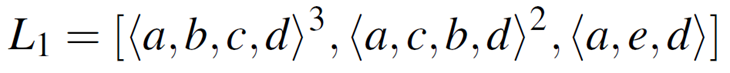
\includegraphics[scale=0.8]{capitolo 2/formula1.png}
        \end{subfigure}
        % Seconda immagine
        \begin{subfigure}{\textwidth}
            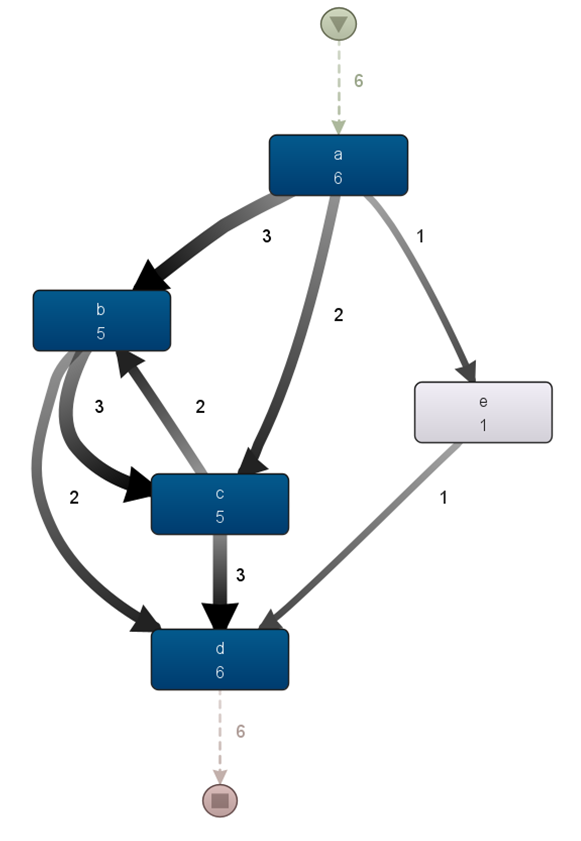
\includegraphics[scale=0.8]{capitolo 2/grafico1.png}
        \end{subfigure}
        % Terza immagine
        \begin{subfigure}{\textwidth}
            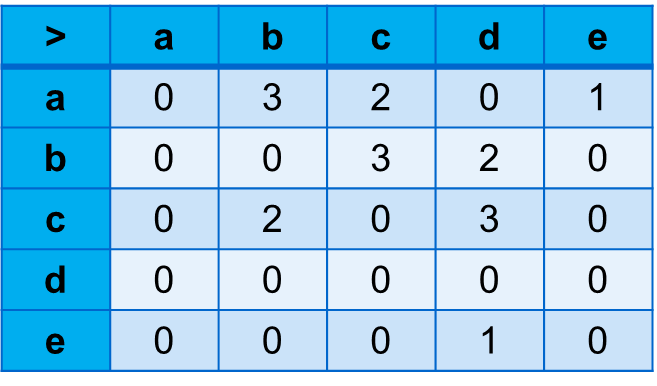
\includegraphics[scale=0.8]{capitolo 2/tabella1.png}
        \end{subfigure}
    \end{figure}
    
    \section{Handling Complexity in Discovery Algorithms}
    
    While the Dependency Graph is a useful way to visualize process flows, it can become unintuitive when certain activities can occur in any order. This is where advanced modeling techniques, such as \textbf{Petri Nets}, come into play. Petri Nets provide a more flexible framework for representing processes where activities may be performed in parallel or in various sequences.
    
    Moreover, processes often include rare or exceptional paths, known as \textbf{infrequent paths}, which may distort the overall representation of the process. These outliers can be filtered out to focus on the \textbf{main stream of behavior}, which represents the most common sequences of activities. By concentrating on the main flow, we gain a clearer picture of the general behavior of the process, while still being able to acknowledge deviations when necessary.
